\label{ch:gradiente}
\chapter[Cálculo del Gradiente]
		{Cálculo del Gradiente}
\section{El gradiente de los armónicos esféricos.}
Para el cálculo del gradiente usaremos una expresión de la base en términos de los polinomios de Gegenbauer. De la proposición \hyperref[]{\ref{geb_rel}}, se deduce que esta base es equivalente a la calculada anteriormente.
\\
\begin{thm}
Sean, $T_{n}(t),U_{n}(t)$ los polinomios de Chebyshev de $1^{er}$ y 2º clase respectivamente.Y definimos
\begin{gather*}
 g_{0,n}(x_1,x_2) = (x_1^2+x_2^2)T_n^2(x_2(x_1^2+x_2^2)^{-1/2})
\\
g_{1,n-1}(x_1,x_2) = x_1(x_1^2+x_2^2)^{\frac{n-1}{2}}U_{n-1}(x_2(x_1^2+x_2^2)^{-1/2})
\end{gather*}
entonces, si tomamos $\textbf{n}=(n_1,...,n_d)$ con $n_1 = \{0,1\}$ se define
\begin{gather*}
Y_\textbf{n} = g_{n_1,n_2}(x_1,x_2)\prod_{j=3}^{d}(x_1^2+...+x_j^2)^{n_j/2}C_{n_j,\lambda_j}(x_j(x_1^2+...+x_j^2)^{-1/2})
\end{gather*}
donde $\lambda_j =\lambda_j(n_1,...,n_{j-1}) = \sum_{i=1}^{j-1}n_i + \frac{j-2}{2}$. Entonces $\{Y_n,|\textbf{n}|=n\}$ es una base de $\mathds{Y}_{n}^{d}$.
\end{thm}
\medskip

Tomamos, $F_n^\lambda (x) = (x_1^2+...+x_j^2)^{n/2}C_{n,\lambda}(\frac{x_d}{\sqrt{(x_1^2+...+x_j^2)}})$.
Si $x=(x_1,...,x_d), n=(n_1,...,n_d)$ y $x' = (x_1,...,x_{d-1}), n=(n_1,..n_{d-1})$.
$Y_n(x) = Y_{n'}(x') F_{n_d}^{\lambda_d} (x)$ siendo $ Y_{n'}(x')$ un esférico armónico de dimensión $d-1$ y grado $n-n_d$.
\begin{prop}Para $i=1,...,d-1$
	\begin{gather*}
	\partial_i  F_{n}^\lambda(x) = -2\lambda x_i F_{n-2}^{\lambda+1}(x) \\ 
	\partial_d F_{n}^{\lambda}(x) = (n+2\lambda-1)  F_{n-1}^{\lambda}(x)
	\end{gather*}
\end{prop}
\begin{proof}
	Sean $r=\sqrt{x_1^2+...+x_d^2},i=1,2,...,d-1$. Usando que $$\frac{d}{dx}C_{n,\lambda}(x) = 2\lambda C_{n-1,\lambda+1}(x)$$ y los apartados $(I)$ y $(II)$ de la Proposición \ref{propGg} entonces
	\begin{gather*}
	\begin{aligned}
	\partial_i F_{n}^{\lambda} &= x_i r^{n-2} \left[ n C_{n,\lambda}(\frac{x_d}{r})-2\lambda\frac{x_d}{r}C_{n+1,\lambda+1}(\frac{x_d}{r})\right] \\&= -2\lambda x_ir^{n-2}C_{n-2,\lambda+1}(\frac{x_d}{r})
	\end{aligned}
	\end{gather*}
	Además,
	\begin{gather*}
		\begin{aligned}
		\partial_d F_{n}^{\lambda}(x) &= r^{n-1}\left[n\frac{x_d}{r}C_{n,\lambda}(\frac{x_d}{r})+2\lambda(1-\frac{x_d^2}{r^2})C_{n-1,\lambda+1}(\frac{x_d}{r})\right] \\&= (n+2\lambda-1)r^{n-1}C_{n-1,\lambda}(\frac{x_d}{r})		
		\end{aligned}
	\end{gather*}
	
	
\end{proof}
Ahora, tomamos la proyección del espacio de los polinomios homogéneos al espacio de los armónicos esféricos $proj_{n,\sphere}^d : \mathds{H}_n^d \to \spharm$ tal que para $P_n\in \mathds{H}_n^d$ verifica 
$$ proj_{n}^d P = \sum_{j=0}^{\lfloor \frac{n}{2} \rfloor}\frac{1}{4^j j! (-n+2-\frac{d}{2})} ||x||^{2j} \triangle^jP
$$
lo que implica que para $Y_\textbf{n}$ se tiene
$$
proj_{n,\sphere}^d (x_iY_{n}(x)) = x_i Y_n(x)-\frac{1}{2(n+(d-2)/2)} ||x||^2 \partial_i Y_n(x)$$
\begin{prop}Sea $n'=|n'|=n-n_d$ e $i=1,2,...,d-1$
	\begin{gather*}
	\begin{aligned}
	\partial_i Y_n(x) &= -2\lambda_d proj_{n'+1,\sphere}^{d-1}(xY_{n'}(x'))F_{n_d-2}^{\lambda_d+1}(x)\\   &+\frac{(n_d+2\lambda_d-1)(n_d+2\lambda_d-2)}{(2\lambda_d-1)(2\lambda_d-2)}\partial_iY_{n'}(x')F_{n_d}^{\lambda_d-1}(x) \\ \quad
	\partial_dY_n(x) &= (n_d+2\lambda_d-1)Y_{n'}(x')F_{n_d-1}^{\lambda_d}(x)
	\end{aligned}
	\end{gather*}
\end{prop}
\begin{proof} Usando los resultados anteriores y que $2\lambda_d-1 = 2n'+d-3$
	$$
	\begin{aligned}\partial_i Y_(x) &= \partial_i Y_{n'}(x')F_{n_d}^{\lambda_d}(x)-2\lambda_d x_i Y_{n'}(x')F_{n_d-2}^{\lambda_d+1}\\ &= -2\lambda_d proj_{n'+1,\sphere}^{d-1}(x_iY_{n'}(x'))F_{n_d-2}^{\lambda_d+1}(x)\\ &+ \partial_iY_{n'}(x')\left[F_{n_d}^{\lambda_d}(x)-\frac{2\lambda_d}{2\lambda_d-1}||x'||^2F_{n_d-2}^{\lambda_d+1}(x)\right]\end{aligned}$$
	Además, como $||x'||^2 = r^2-x_d^2$ y en virtud de los apartados $(I)$ y $(IV)$ de la proposición \ref{propGg}
	$$\begin{aligned}
	F_{n_d}^{\lambda_d}(x) -\frac{2\lambda_d}{2\lambda_d-1}||x'||^2F_{n_d-2}^{\lambda_d+1}(x) &=   r^n_d\left[C_{n_d}^{\lambda}(\frac{x_d}{r}) - -\frac{2\lambda_d}{2\lambda_d-1}(1-\frac{x_d}{r^2})C_{n_d-2}^{\lambda_d+1}(\frac{x_d}{r})\right] \\ &=   \frac{(n_d+2\lambda_d-1)(n_d+2\lambda_d-2)}{(2\lambda_d-1)(2\lambda_d - 2)}r^{n_d}C_{n_d}^{\lambda_d-1}(\frac{x_d}{r})
	\end{aligned}
	$$
	Sustituyendo esta igualdad en la obtenida anteriormente, se prueba el resultado.
\end{proof}
\begin{prop}Sea $n'=|\textbf{n}'|=n-n_d$ e $i=1,...,d-1$
	\begin{gather*}
	\begin{aligned}
		proj_{n+1,\sphere}^d(x_iY_n(x)) &= \frac{\lambda_d}{n_d+\lambda_d} proj_{n'+1,\sphere}^{d+1}(x_iY_{n'}(x'))F_{n_d}^{\lambda_d +1}(x)+\\& \frac{(n_d+1)(n_d+2)}{(2\lambda_d-1)(2\lambda_d-2)2(n_d+\lambda_d)}\partial_iY_{n'}(x')F_{n_d+2}^{\lambda-1}(x)\\
		proj_{n+1,\sphere}^d(x_dY_n(x)) &= \frac{n_d+1}{2(n_d+\lambda_d)}Y_{n'}(x')F_{n_d+1}^{\lambda_d}(x)
	\end{aligned}
	\end{gather*}
\end{prop}
\begin{proof}
	$$proj_{n+1,\sphere}^d(x_iY_n(x)) = x_iY_{n'} F_{n_d}^{\lambda_d}(x)-\frac{r^2}{2(n_d+\lambda_d)}\partial_i(Y_{n'}(x')F_{n_d}^{\lambda_d}(x))$$
	Usando la Proposición 2.3 tenemos que
	\begin{gather*}
	\begin{aligned}
	&proj_{n+1,\sphere}^d(x_iY_n(x))= \\ & proj_{n'+1,\sphere}^{d-1}(x_iY_{n'}(x'))\left[F_{n_d}^{\lambda_d}+\frac{\lambda_d}{n_d+\lambda_d}r^2F_{n_d-2,\lambda_d+1}(x)\right]\\&+\partial_iY_{n'}(x')\left[\frac{||x'||^2}{2\lambda_d-1}F_{n_d}^{\lambda_d}(x)-\frac{(n_d+2\lambda_d-1)(n_d+2\lambda_d)-2}{2(n_d+\lambda_d)(2\lambda_d-1)(2\lambda_d-2)}r^2F_{n_d}^{\lambda_d-1}(x)\right]
	\end{aligned}
	\end{gather*} 
	
	Ahora, aplicando el apartado $(IV)$ de la Proposición \ref{propGg}
	\begin{gather*}
	\begin{aligned}
	F_{n_d}^{\lambda_d}+\frac{\lambda_d}{n_d+\lambda_d}r^2F_{n_d-2,\lambda_d+1}(x) &= r^{n_d}\left[C_{n_d}^{\lambda_d}(\frac{x_d}{r})+\frac{\lambda_d}{n_d+\lambda_d}C_{n_d-2}^{\lambda_d+1}(\frac{x_d}{r})\right] \\&= \frac{\lambda_d}{n_d+\lambda_d}r^{n_d}C_{n_d}^{\lambda_d+1}(\frac{x_d}{r})
	\end{aligned}
	\end{gather*}
	Por otro lado, aplicando el apartado $(I)$ de la Proposición \ref{propGg}
	\begin{gather*}
	\begin{aligned}
	&\frac{||x'||^2}{2\lambda_d-1}F_{n_d}^{\lambda_d}(x)-\frac{(n_d+2\lambda_d-1)(n_d+2\lambda_d)-2}{2(n_d+\lambda_d)(2\lambda_d-1)(2\lambda_d-2)}r^2F_{n_d}^{\lambda_d-1}(x) \\&= \frac{r^{n_d+2}}{2\lambda_d-1}\left[(1-\frac{x_d^2}{r^2})C_{n_d}^{\lambda_d}(\frac{x_d}{r})-\frac{(n_d+2\lambda_d-1)(n_d+2\lambda_d-2)}{2(n_d+\lambda_d)(2\lambda_d-2)}C_{n_d}^{\lambda_d - 1}(\frac{x_d}{r})\right] \\ &= \frac{(n_d+1)(n_d+2)}{2(n_d+\lambda_d)(2\lambda_d-1)(2\lambda_d-2)}r^{n_d+2}C_{n_d+2}^{\lambda_d-1}(\frac{x_d}{r})
	\end{aligned}
	\end{gather*}
	Uniendo ambas igualdades se prueba la primera igualdad de la proposición.
	\\Finalmente,
	\begin{gather*}
	\begin{aligned}
	&proj_{n+1,\sphere}^d(x_dY_n(x)) = x_dY_{n'}(x')F_{n_d}^{\lambda_d}(x)-\frac{r^2}{2(n_d+\lambda_d)}\partial_d(Y_{n'}(x')F_{n_d}^{\lambda_d}(x)) \\&=Y_{n'}(x')\left[x_dF_{n_d}^{\lambda_d}(x)-\frac{r^2}{2(n_d+\lambda_d)}(n_d+2\lambda_d-1)F_{n_d-1}^{\lambda_d}(x)\right] \\&= \frac{n_d+1}{2(n_d+\lambda_d)}Y_{n'}(x')F_{n_d+1}^{\lambda_d}(x)
	\end{aligned}
	\end{gather*}
\end{proof}
\begin{thm}
	Sea $n=(n_1,n_2,...,n_d)\in\mathds{N}_0^d$ con $n_1=\{0,1\}$ y $|n|=n$. Entonces
	$\partial_i Y_n(x)$ es un esférico armónico de grado n-1 $$
	<\partial_i Y_n,Y_m>_{\sphere} \neq 0 \quad |m|=n-1$$
	para sólo $2^{d-2}$ índices, $m\in\mathds{N}_0^d$ con $m_1=\{0,1\}$
\end{thm}
\begin{proof}
La afirmación del teorema equivale a $\partial_i Y_n = \sum_{m} a_mY_m^{n-1}$ siendo $a_m$ una constante real. El resultado se prueba por inducción sobre la dimensión $d$ usando las proposiciones anteriores.
Para $d=2$, 
\begin{gather*}
\begin{aligned}
\partial_1 Y_n^{(1)}(x) &= nY_{n-1}^{(1)}(x) \qquad \partial_2 Y_n^{(1)}(x) = -nY_{n-1}^{(2)}(x)
\\ \partial_1 Y_n^{(2)}(x) &= nY_{n-1}^{(2)}(x) \qquad \partial_2 Y_n^{(2)}(x) = nY_{n-1}^{(1)}(x)
\end{aligned}
\end{gather*}
Supongamos cierto el resultado para dimensión $d-1$. Entonces $\partial_i Y_{n'}(x')$ puede escribirse como combinación lineal de a lo sumo $2^{d-3}$ esféricos $Y_m'^{n'-1}$. Como $Y_m^{n'-1}F_{n_d}^{\lambda_d-1} = Y_{m_1,...m_{d-1},n_d}^{n-1}$, el resultado se obtiene aplicando la Proposición 2.2.
\end{proof}
\subsection{Caso particular d=3}
El espacio de los esféricos armónicos de grado n en dimensión 3 tiene dimensión 2n+1. Tomando coordenadas esféricas,
\begin{gather*}
\begin{aligned}
x_1 &= r \sen \theta \sen \phi\\
x_2 &= r \sen \theta \sen \phi\\
x_3 &= r \cos \theta\\
\end{aligned}
\\
0\le \theta \le \pi,0\le\phi\le2\pi,r>0
\end{gather*}
una base ortogonal de $\spharm$ viene dada por
\begin{equation}
	\left\lbrace
	\begin{array}{ll}
	Y^n_ {k,1} = r^n(\sen \theta)^kC_{n-k,k+1/2}(\cos \theta) \cos(k\phi),\quad 0\le k\le n \\
	Y^n_{k,2}(x) = r^{n-k}(\sen\theta)^kC_{n-k,k+1/2}(\cos\theta)\sen(k\phi), \quad 1\le k\le n
	\end{array}
	\right.
\end{equation}

\begin{prop} Para $k=0,...,n$
	\begin{gather*} 
		\begin{aligned}
			\partial_1Y^{n}_{k,1}(x) &= -\frac{(n+k)(n+k-1)}{2(2k-1)}Y^{n-1}_{k-1,2}(x)-(k+\frac{1}{2})Y^{n-1}_ {k+1,2}(x) \\
		\partial_2Y^{n}_{k,1}(x) &= \frac{(n+k)(n+k-1)}{2(2k-1)}Y^{n-1}_{k-1,1}(x)-(k+\frac{1}{2})Y^{n-1}_ {k+1,1}(x) \\
		\partial_3 Y_{k,1}^{n}(x) &=(n+k)Y_{k,1}^{n-1}(x)
			\end{aligned}
	\end{gather*}
 Para $k=1,...,n$
	\begin{gather*}
	\begin{aligned}
	\partial_1Y^{n}_{k,2}(x) &= \frac{(n+k)(n+k-1)}{2(2k-1)}Y^{n-1}_{k-1,1}(x)+(k+\frac{1}{2})Y^{n-1}_ {k+1,1}(x)\\
	\partial_2Y^{n}_{k,2}(x) &= \frac{(n+k)(n+k-1)}{2(2k-1)}Y^{n-1}_{k-1,2}(x)-(k+\frac{1}{2})Y^{n-1}_ {k+1,2}(x)\\
	\partial_3 Y_{k,2}^{n}(x) &=(n+k)Y_{k,2}^{n-1}(x)
		\end{aligned}
	\end{gather*}
\end{prop}
\section{Puntos críticos del gradiente.}
Finalmente, queremos conocer el número de puntos que anulan el gradiente, para ello haremos uso de las siguientes igualdades trigonométricas
\begin{gather*}
\begin{aligned}
\cos(k\phi) &= \sen(k\phi + \frac{\pi}{2}) \\
\sen (k\phi) &= \cos(k\phi - \frac{\pi}{2}) \\
\cos(k+1)\phi &= \cos (k\phi)\cos\phi - \sen k\phi \sen\phi \\
\cos(k-1)\phi &= \cos (k\phi)\cos\phi + \sen k\phi \sen\phi \\
\sen(k+1)\phi &= \sen(k\phi)\cos\phi + \sen(\phi)\cos(k\phi)\\
\sen(k-1)\phi &= \sen(k\phi)\cos\phi - \sen(\phi)\cos(k\phi)\\
\end{aligned}
\end{gather*}
Llamaremos  $c_{n,k},d_k$ a las constantes $\frac{(n+k)(n+k-1)}{2(2k-1)},k+\frac{1}{2}$ respectivamente
Igualando a 0 las parciales calculadas anteriormente tenemos que para $k\ge0$
\begin{gather}
\partial_3 Y_{k,1}^n(x) = (n+k)Y_{k,1}^{n-1}(x) = (n+k)(\sen \theta)^k C_{n-k-1,k+1/2}(\cos \theta) \cos k\phi = 0
\end{gather}
implica que ha de verificarse una de las siguientes igualdades
\begin{gather}
\left\{
\begin{array}{ll}
\sen \theta= 0 \\
\cos k\phi = 0\\
C_{n-k-1,k+1/2}(\cos \theta) = 0
\end{array}
\right.
\end{gather}
Si $\sen \theta = 0$ tendremos que $\theta=0$ o $\theta=\pi$.
\medskip

Ahora, suponemos que $\cos k\phi = 0 $, entonces
\begin{gather}
\begin{aligned}
 \partial_1  Y_{k,1}^n(x) &= (\sen\theta)^{k-1}[-c_{n,k}C_{n-k,k-1/2}(\cos \theta)\sen(k\phi)\cos\phi \\&+ d_k \sen^2\theta C_{n-k-2,k+3/2}(\cos \theta)\sen(k\phi)\cos\phi] \\ &= (\sen\theta)^{k-1}\sen(k\phi)\cos\phi[-c_{n,k}C_{n-k,k-1/2}(\cos \theta) 
\\&+ d_k \sen^2\theta C_{n-k-2,k+3/2}(\cos \theta)]
\end{aligned}
\end{gather}
\begin{gather}
\begin{aligned}
\partial_2  Y_{k,1}^n(x) &= (\sen\theta)^{k-1}[-c_{n,k}C_{n-k,k-1/2}(\cos \theta)\sen(k\phi)\sen\phi \\&+ d_k \sen^2\theta C_{n-k-2,k+3/2}(\cos \theta)\sen(k\phi)\sen\phi] \\ &= (\sen\theta)^{k-1}\sen(k\phi)\sen\phi[-c_{n,k}C_{n-k,k-1/2}(\cos \theta) \\&+ d_k \sen^2\theta C_{n-k-2,k+3/2}(\cos \theta)]
\end{aligned}
\end{gather}
Ahora, igualando ambas expresiones a 0
\begin{gather}
\begin{aligned}
	\partial_1  Y_{k,1}^n(x) &= \partial_2  Y_{k,1}^n(x)  \\ &= (\sen\theta)^{k-1}\sen(k\phi)\cos\phi[c_{n,k}C_{n-k,k-1/2}(\cos \theta) + d_k \sen^2\theta C_{n-k-2,k+3/2}(cos \theta)]  \\ &= (\sen\theta)^{k-1}sen(k\phi)\sen\phi[c_{n,k}C_{n-k,k-1/2}(\cos \theta) + d_k \sen^2\theta C_{n-k-2,k+3/2}(\cos \theta)] \\ &= 0
\end{aligned}
\end{gather}
Como $cos (k	\phi) = 0 $ entonces $sen  (k\phi) \neq 0$. Además, $sen \phi$ y $cos\phi$ no se anulan simultáneamente, luego de la expresión anterior se verifica que
\begin{gather*}
c_{n,k}C_{n-k}^{k-1/2}(cos \theta) + d_k sen^2\theta C_{n-k-2}^{k+3/2}(cos \theta) = 0
\end{gather*}
Haciendo el cambio $sen^2 \theta = 1-cos^2\theta$, y tomando como variable $t=cos\theta$, se tiene que la expresión anterior es un polinomio de grado a lo sumo $n-k$. Por tanto, tiene a lo sumo $n-k$ raíces.

\medskip

Consideremos el polinomio:

\begin{gather*}
Q_{n,k}(t) =(n-k)(n+k-1)C_{n-k,k-\frac{1}{2}}(t)+(2k-1)(1-t^2)C_{n-k-2,k+\frac{3}{2}}(t)
\end{gather*}
De la ecuación (I) de la Proposición \ref{propGg} deducimos que:
\begin{gather*}
(2k-1)(2k+1)C_{n-k-2,k+\frac{3}{2}}(t) = \left(C_{n-k,k-\frac{1}{2}}\right)'' (t)
\end{gather*}

De la ecuación diferencial de los polinomios de Gegenbauer (Proposición \ref{Ggdif}) obtenemos:
\begin{gather*}
(1-t^2)\left(C_{n-k,k-\frac{1}{2}}\right)'' (t) = 2kt\left(C_{n-k,k-\frac{1}{2}}\right)'(t)-(n-k)(n-k-1)C_{n-k,k-\frac{1}{2}}(t)
\end{gather*}

Por tanto,
\begin{gather*}
\begin{aligned}
Q_{n,k}(t) &= \left[(n+k)(n+k-1)-(n-k)(n+k-1)\right] C_{n-k,k-\frac{1}{2}}(t) \\&+ 2kt\left(C_{n-k,k-\frac{1}{2}}\right)'(t) \\&= 2k\left[(n+k-1)C_{n-k,k-\frac{1}{2}}(t)+ t\left(C_{n-k,k-\frac{1}{2}}\right)'(t)\right]
\end{aligned}
\end{gather*}
y usando de (III) en la Proposición \ref{propGg} queda
\begin{gather*}
Q_{n-k}(t) = 2k\left(C_{n-k+1,k-\frac{1}{2}}\right)'(t)
\end{gather*}
que tiene exactamente $n-k$ raíces reales y distintas contenidas en el intervalo $[1,-1]$.

En resumen, hemos encontrado $2k(n-k)+2$ valores que anulan las 3 parciales.

\medskip
Razonando análogamente, se obtiene la misma conclusión para las parciales de los armónicos esféricos del segundo tipo.

\bigskip

A continuación, se muestran algunos ejemplos de los puntos críticos obtenidos para distintos valores de $n$ y $k$.
\begin{figure}[H]
	\centering
	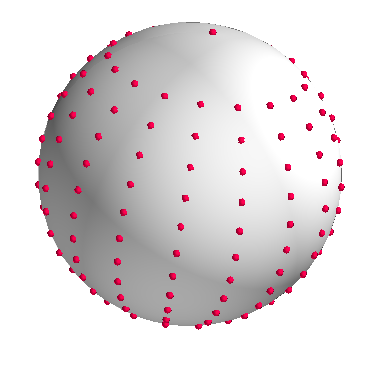
\includegraphics[scale=0.5]{img/gradient_20_9.png}
	\caption{Puntos críticos del gradiente para n=20 y k=9.}
\end{figure}

\begin{figure}[H]
	\centering
	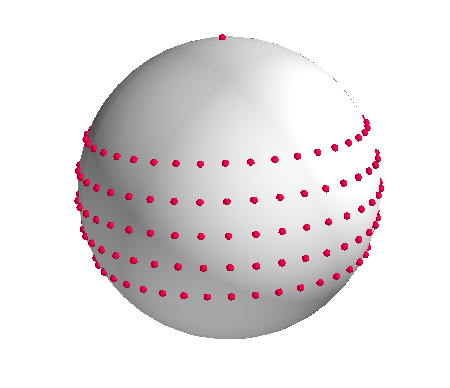
\includegraphics[scale=0.5]{img/gradient_25_5.png}
	\caption{Puntos críticos del gradiente para n=25 y k=20.}
\end{figure}

\begin{figure}[H]
	\centering
	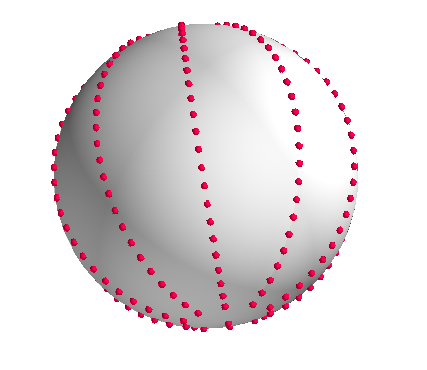
\includegraphics[scale=0.5]{img/gradient_30_5.png}
	\caption{Puntos críticos del gradiente para n=30 y k=5.}
\end{figure}
